\documentclass{article}
\usepackage{amsmath}

\usepackage{Sweave}
\begin{document}
\Sconcordance{concordance:SymmetricRandomWalk.tex:SymmetricRandomWalk.Rnw:%
1 6 1 50 0 9 1 8 0 28 1 1 13 6 1 1 5 11 1 1 19 24 1}


\section{Description}
The symetric random walk will be described in this document (Mt). it covers the theory of "Stochastic Calculus for finance" Tome 2 chapter 3 section 1.

The construction of the random walk depend on the evolution of a random variable $X_i$. The previous RV can take two value at each time, like tossing a coin. $X_i$ can take the value 1 or -1.

\begin{equation}
 \label{eq:Xi}
X_i = 
\left \{{
  \begin{array}{c} 1 \\ -1 \end{array}
  }\right .
\end{equation}
 
The Symetric Random Walk is constructed by summing up the different outcome of the random variable $X_i$ from $k$ experiments:

\begin{equation}
\label{eq:SRW}
M_k = 
\sum_{j=1}^k X_j
\end{equation}

In the following lines of code, $X_i$ is randomly difined. The variable $k$ ensure to have a sufficent number of periods to further generate the scaled random walk.
It refers to the $k$ of equation~\ref{eq:SRW}.
$p$ and $q$ are the probability measure, respectively $p$ chance to get value 1 and $q$ chance to get -1 from random variable $X_i$.




After creating the random variable $X_i$ it suffices to add up all the differente output we get from time 1 up to $k$ to get a specific Symetric Random Walk.

The following outcome present a randomly generated 300 steps symmetric random walk.

\begin{table}[h]
0 1 2 3 4 3 2 1 2 3 2 1 2 1 0 1 2 3 4 5 4 5 4 3 2 1 0 -1 -2 -3 -2 -3 -4 -3 -2 -3 -4 -5 -4 -3 -4 -5 -6 -7 -6 -7 -8 -9 -8 -9 -8 -7 -6 -5 -4 -3 -4 -5 -6 -7 -6 -5 -6 -5 -4 -5 -4 -3 -4 -5 -6 -7 -6 -5 -6 -7 -6 -5 -4 -3 -4 -3 -4 -5 -6 -7 -6 -5 -6 -7 -6 -5 -4 -3 -4 -3 -4 -5 -4 -5 -4 -5 -6 -7 -8 -9 -8 -7 -8 -9 -10 -11 -12 -13 -14 -15 -16 -15 -14 -15 -16 -17 -16 -15 -14 -15 -16 -15 -16 -17 -18 -19 -18 -17 -16 -15 -16 -17 -16 -15 -16 -17 -18 -17 -18 -19 -20 -21 -22 -23 -24 -23 -22 -23 -22 -23 -24 -23 -22 -21 -22 -23 -24 -23 -24 -23 -24 -23 -24 -25 -26 -27 -28 -29 -30 -29 -30 -29 -28 -29 -28 -27 -28 -27 -28 -27 -26 -27 -28 -27 -26 -27 -28 -29 -28 -29 -30 -31 -30 -29 -30 -31 -32 -31 -30 -31 -30 -29 -30 -31 -32 -33 -34 -33 -32 -31 -32 -31 -32 -31 -30 -29 -28 -27 -28 -27 -26 -25 -24 -23 -24 -25 -24 -23 -24 -25 -26 -25 -26 -27 -28 -27 -26 -27 -28 -29 -30 -29 -30 -29 -30 -31 -30 -31 -30 -29 -28 -29 -28 -27 -28 -29 -28 -27 -26 -25 -24 -23 -22 -23 -24 -23 -22 -23 -22 -21 -22 -23 -24 -25 -26 -25 -26 -25 -26 -27 -28 -27 -28 -27 -26 -27 -28 -29 -30 -31 -30 -31 -30 -31 -32\caption{300 steps Symmetric Random Walk}
\end{table}


\begin{figure}[!h]
\begin{center}


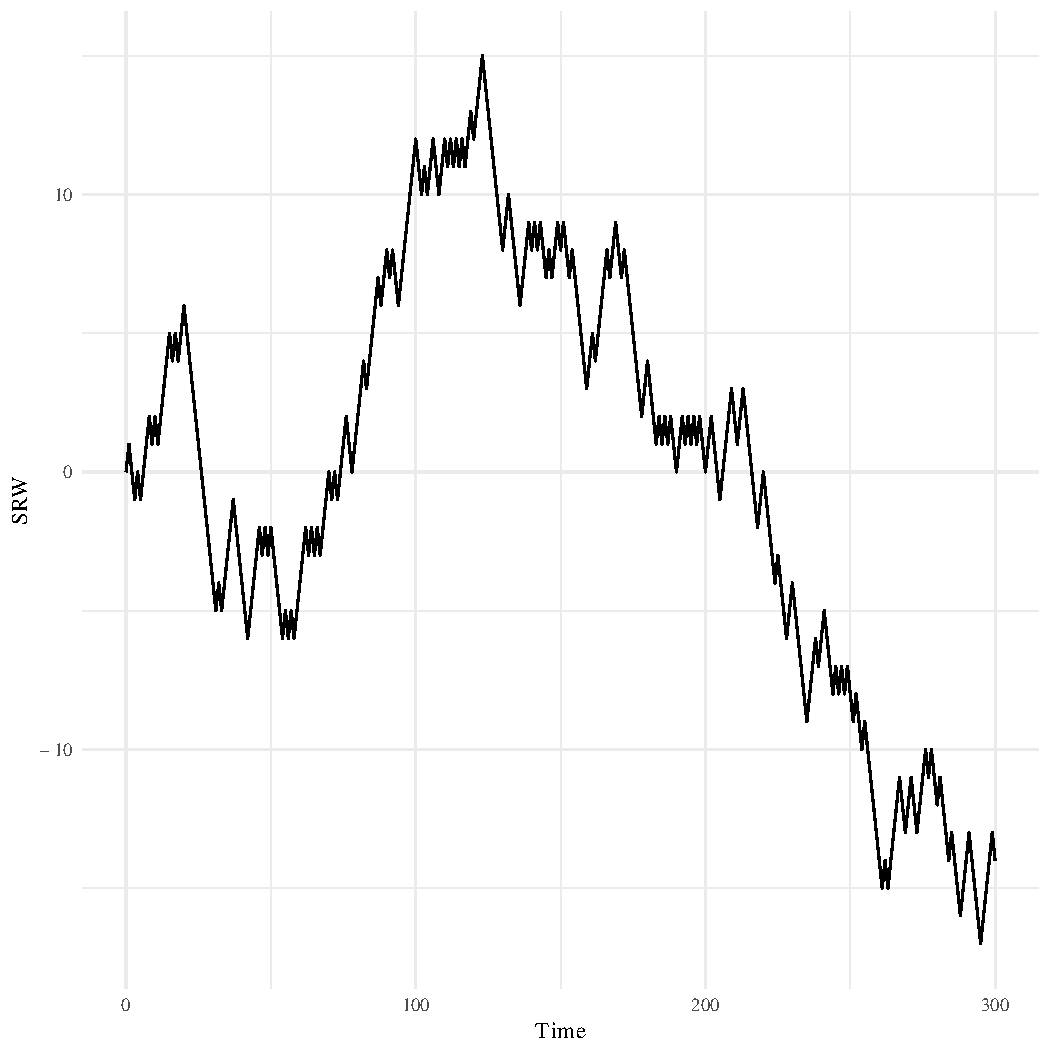
\includegraphics[width=1.0\textwidth]{SRW.pdf}

\end{center}
\caption{Symmetric Random Walk}
\end{figure}

















\end{document}
